\section{Resultados y Análisis}
\begin{frame}[t]
\frametitle{Resultados y Análisis}

En este capítulo se describen ciertos pasos y funcionamientos de la solución en general, para esto se supone una habitación con un sensor de temperatura, un ventilador y un bombillo led, las cuales el usuario va a visualizar y gestionar desde la aplicación web. En la figura \ref{fig:iot} está el esquema del sistema IoT.

\begin{figure}
	\centering
	\caption{Esquema Solución SmartHouse [Imagen Propia]}
	\label{fig:iot}
	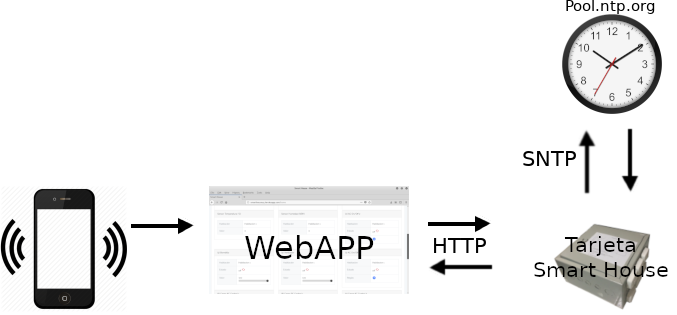
\includegraphics[width=0.6\linewidth]{Imagenes/IOT}
\end{figure}
\end{frame}

\subsection{Software}
\begin{frame}[t]
\frametitle{Resultados y Análisis}
\framesubtitle{Software}

Se desarrolla la aplicación web de manera local y posteriormente se lanza a un servidor en Internet. Se encuentra compuesta por los siguientes sitios y las diferentes interacciones basadas en las funciones básicas crear, leer, actualizar y borrar (CRUD).

\begin{itemize}
	\item Parte Pública
	\item Parte Privada
	\begin{itemize}
		\item Intercambio de datos
		\item Panel de Control
		\begin{itemize}
			\item Crear
			\item Ver
			\item Editar
			\item Eliminar 
		\end{itemize}
	\end{itemize}
\end{itemize}

\end{frame}

\begin{frame}[t]
\frametitle{Resultados y Análisis}
\framesubtitle{Software}
\footnotesize
De acuerdo con la lista anterior, se toman en cuenta dos partes, una pública y una privada, como se observa en la figura \ref{fig:index}. En la parte pública se encuentra una vista con la información de contacto del fabricante, solicitudes de registro o productos y la cantidad de usuarios que actualmente estan registrados en la aplicación. En la parte privada se encuentra la interacción de los usuarios sea administrador, dueño de una casa o de una habitación, para controlar y observar sus datos.

\begin{figure}
	\centering
	\caption{Página de Inicio. [Imagen Propia]}
	\label{fig:index}
	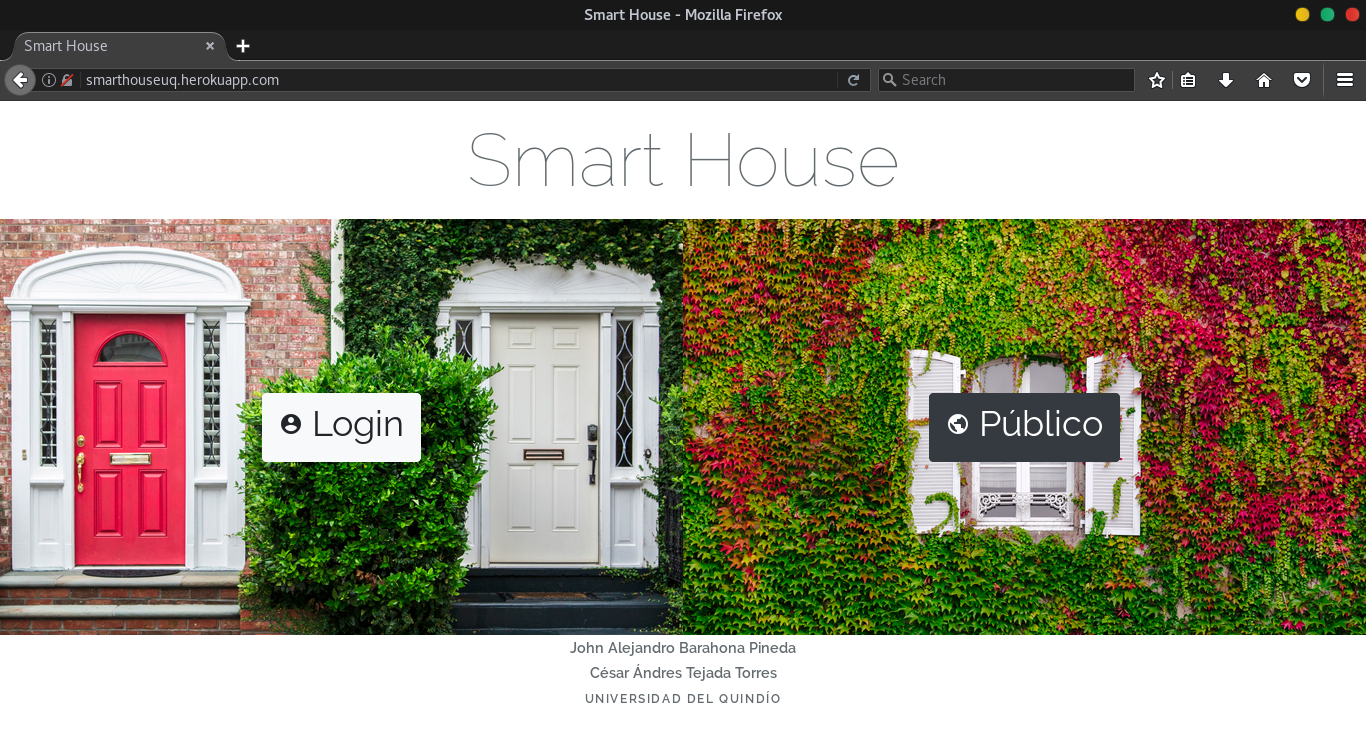
\includegraphics[width=0.6\linewidth]{Imagenes/Index}
\end{figure}

\end{frame}

\subsubsection{Parte Pública}

\begin{frame}[t]
\frametitle{Resultados y Análisis}
\framesubtitle{Software | \emph{Parte Pública}}

En esta vista únicamente hay opciones para el contacto y solicitudes, como se menciona anteriormente, es sencilla debido a la poca información que contiene, según se observa en la figura \ref{fig:publicview}.

\begin{figure}[H]
\centering
\caption{Vista Pública. [Imagen Propia]}
\label{fig:publicview}
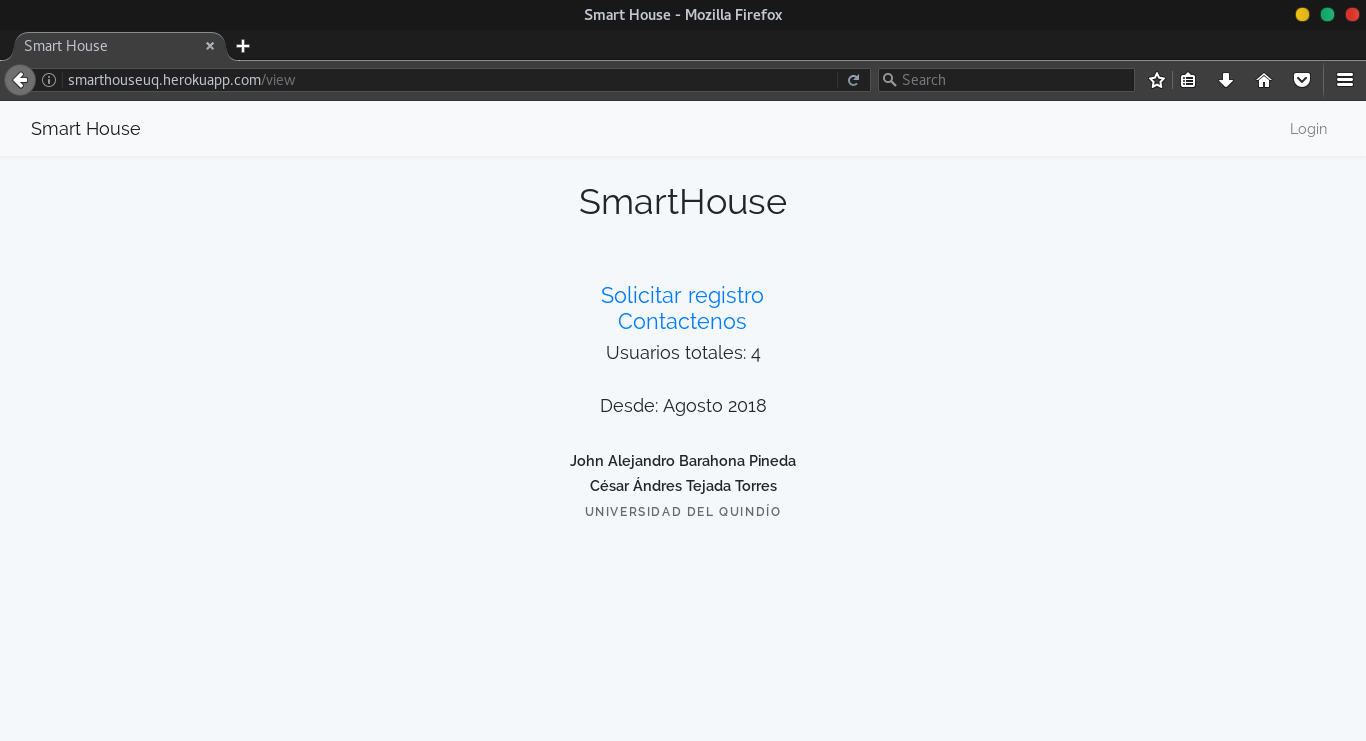
\includegraphics[width=0.5\linewidth]{Imagenes/Public_view}
\end{figure}

\end{frame}

\subsubsection{Parte Privada}

\begin{frame}[t]
\frametitle{Resultados y Análisis}
\framesubtitle{Software | \emph{Parte Privada}}
\begin{wrapfigure}{r}{0.5\linewidth}
	\centering
	\caption{Vista Usuario Administrador. [Imagen Propia]}
	\label{fig:adminview}
	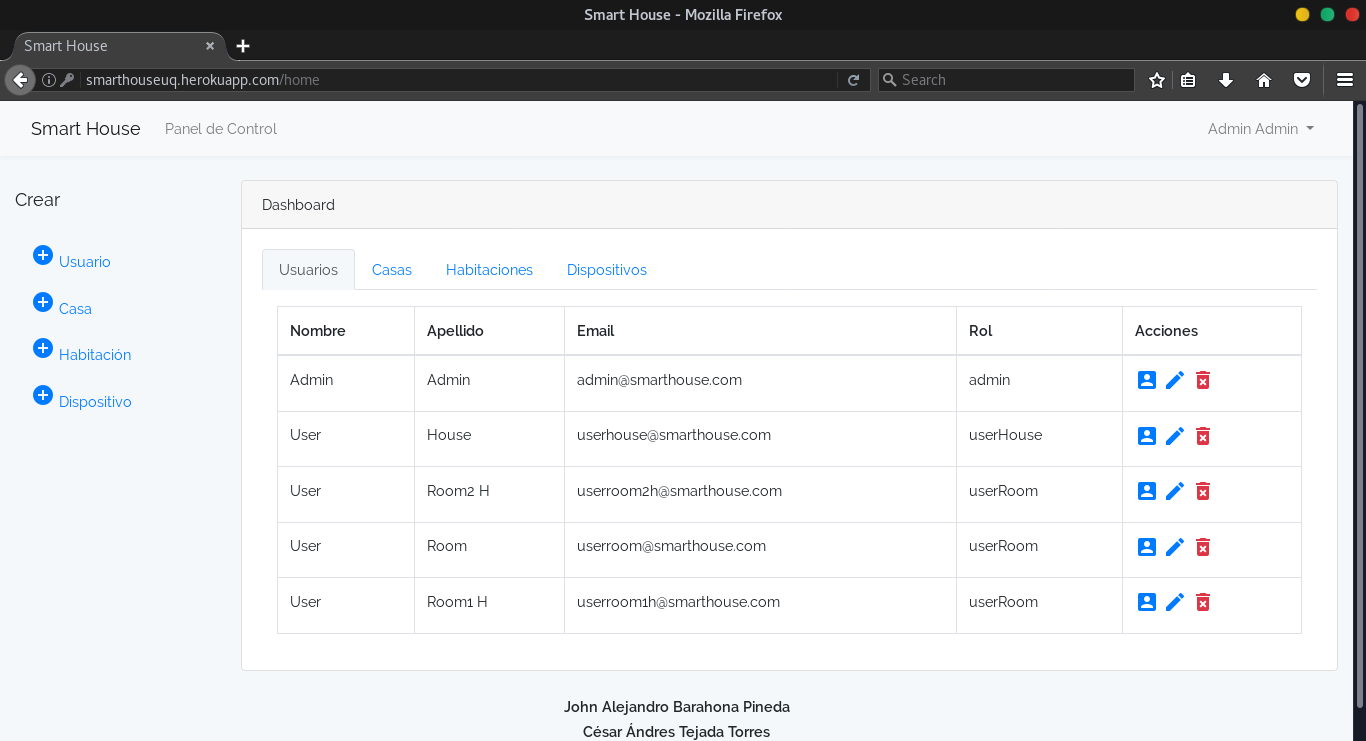
\includegraphics[width=\linewidth]{Imagenes/Admin_view}
\end{wrapfigure}
En esta sección es donde se encuentra el Panel de Control para los diferentes usuarios de la aplicación. En primera instancia, un usuario administrador, el cual esta encargado de gestionar la aplicación, tiene la posibilidad de crear, ver, editar y eliminar los registros de la aplicación, la vista de este usuario se puede observar en la figura \ref{fig:adminview}. Por medio de este se activan las cuentas de los demás, razón por la cual en la parte pública están las opciones de contacto y solicitud de registro.
\end{frame}


\begin{frame}[t]
\frametitle{Resultados y Análisis}
\framesubtitle{Software | \emph{Parte Privada}}
\begin{wrapfigure}{r}{0.5\linewidth}
	\centering
	\caption{Vista Usuario de Casa. [Imagen Propia]}
	\label{fig:houseview}
	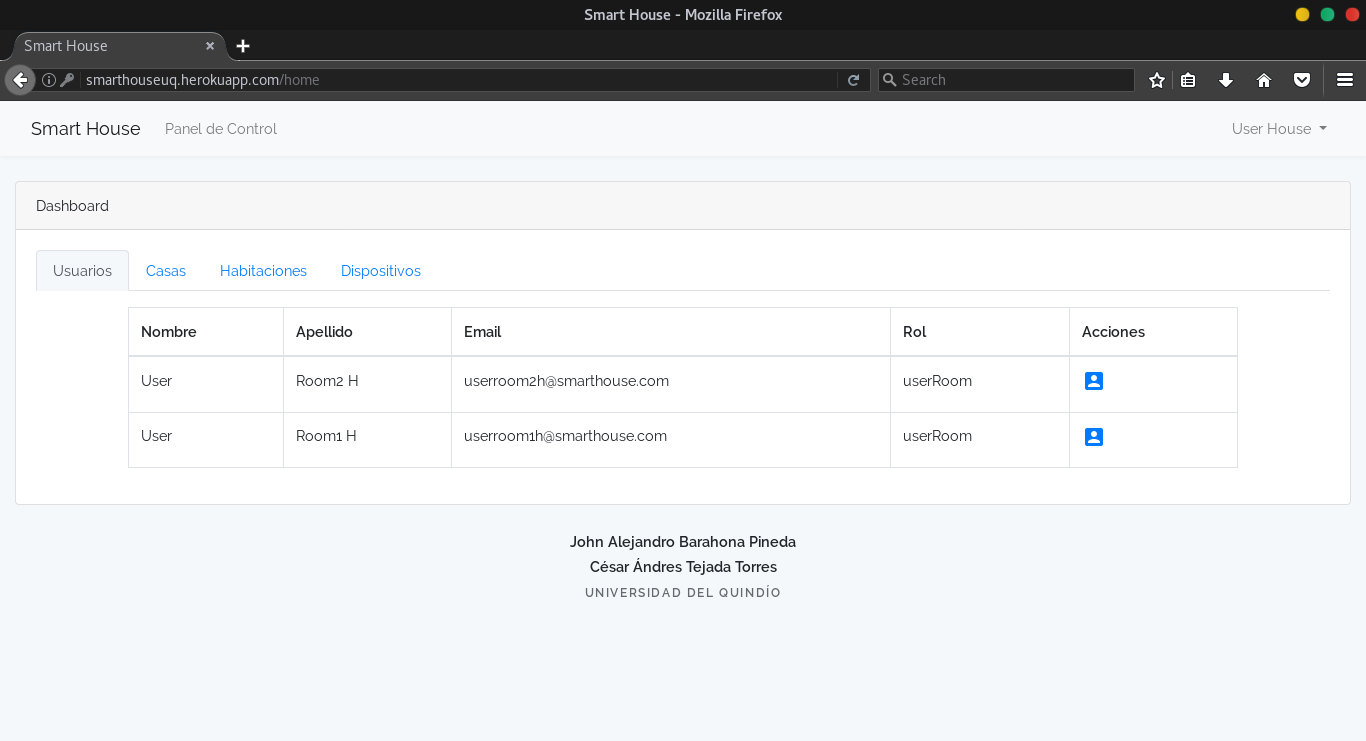
\includegraphics[width=\linewidth]{Imagenes/UserH_view}
\end{wrapfigure}
También existe el usuario dueño de la vivienda donde se encuentra el dispositivo, este es opcional y es para gestionar los dispositivos presentes dentro de un mismo domicilio, es un administrador de la casa, el cual puede revisar y editar algunos campos de sus usuarios hijos o usuarios habitación y sus diferentes casas y habitaciones registradas a su nombre, como se ve en la figura \ref{fig:houseview}, de este modo el rol de dicho usuario es administrar su hogar y visualizar los datos de esta.
\end{frame}

\begin{frame}[t]
\frametitle{Resultados y Análisis}
\framesubtitle{Software | \emph{Parte Privada}}

\begin{wrapfigure}{r}{0.5\linewidth}
	\centering
	\caption{Vistas de Usuario Habitación [Imagen Propia]}
	\label{fig:userview}
	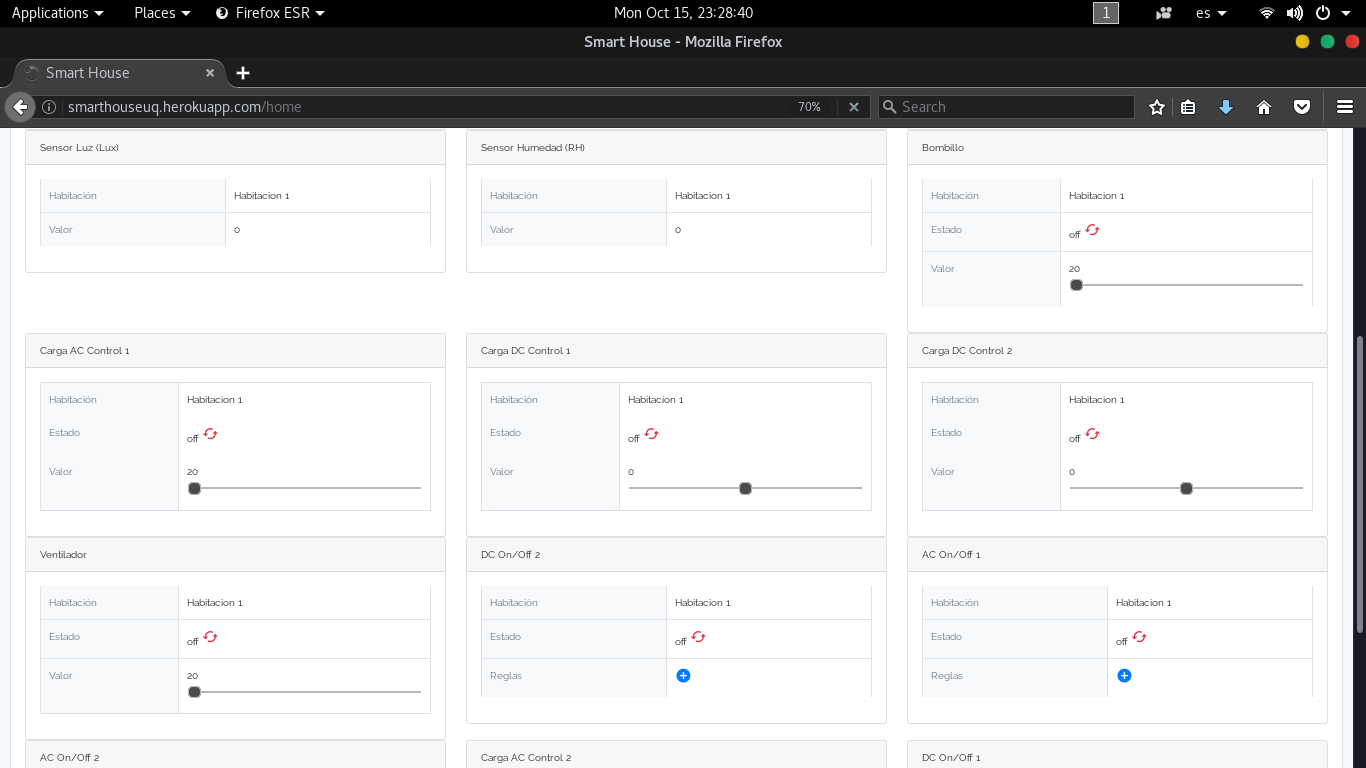
\includegraphics[width=\linewidth]{Imagenes/UserR_view}
\end{wrapfigure}
Por último, otro rol es el de usuario habitación, el cuál únicamente visualiza sus propios datos, como la habitación y los dispositivos presentes en esta, según se observa en la figura \ref{fig:userview}, a este solo le compete la información de lo que posee en su cuarto, por tal motivo el panel de control muestra una vista general de los datos y el estado de sus dispositivos, además de tener la capacidad de editar partes básicas de su habitación y perfil. Dicho usuario puede o no estar sujeto a un usuario padre o usuario casa, ya que, solamente posee una tarjeta para su habitación y ninguna otra en dicha casa.

\end{frame}

\begin{frame}[t]
\frametitle{Resultados y Análisis}
\framesubtitle{Software | \emph{Parte Privada}}
\footnotesize 
\begin{wrapfigure}{r}{0.5\linewidth}
	\centering
	\caption{Página de intercambio de datos [Imagen Propia]}
	\label{fig:updateview}
	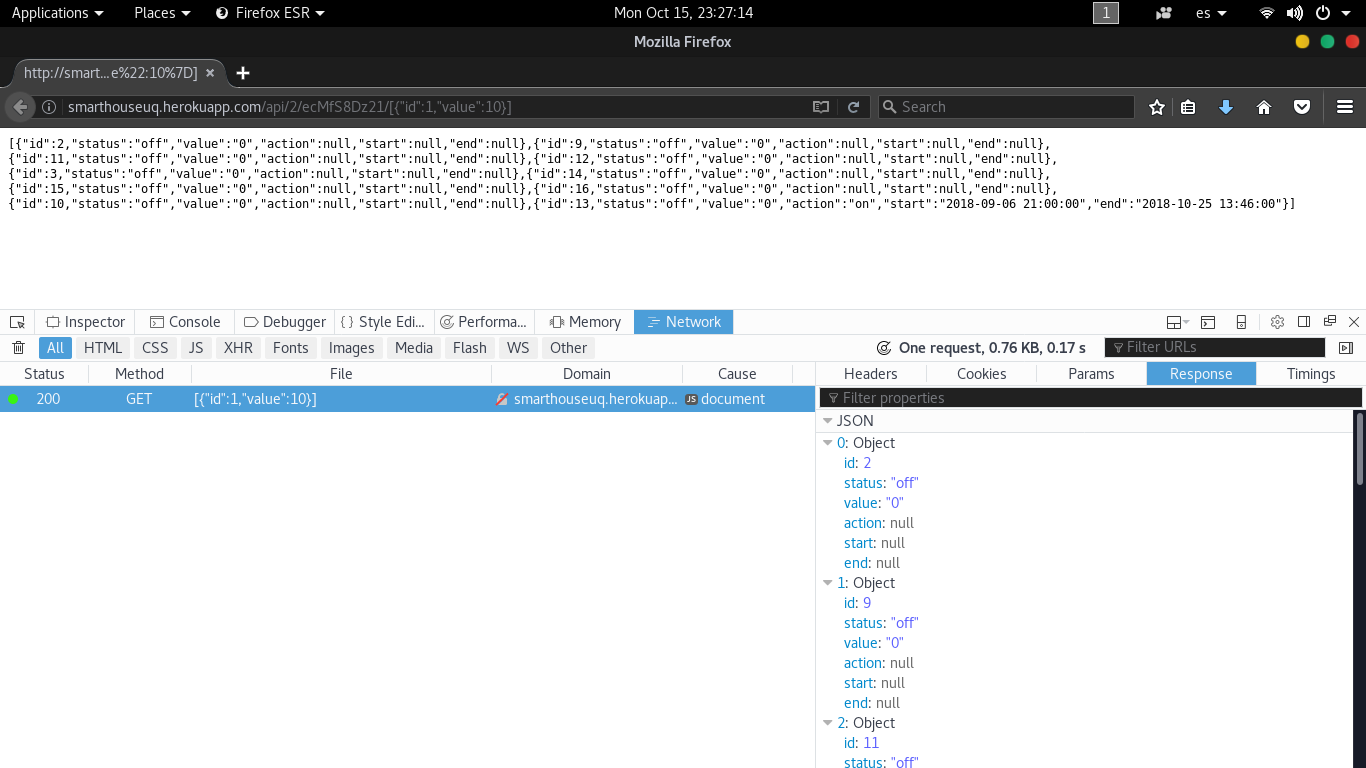
\includegraphics[width=0.9\linewidth]{Imagenes/Update_view}
\end{wrapfigure}
En la parte privada también se encuentra la ruta encargada de la actualización Servidor-Tarjeta, es decir, en esta ruta es donde se intercambia la información. Allí se realiza una petición HTTP tipo GET por parte de la tarjeta, incluyendo en su contenido el id de la habitación en la que está instalada, junto con el token correspondiente a esta, además en la URL se añade un texto tipo JSON en el cual se ubican todas los datos de la lectura actual de los sensores; esta petición la responde el servidor con un texto también tipo JSON que contiene la información pertinente de las cargas o actuadores como se observa la figura \ref{fig:updateview}, para dar seguridad a dicha transacción, se utiliza un token, el cual se verifica mediante el id de la habitación comparando el recibido con el almacenado.

\end{frame}

\begin{frame}
\frametitle{Resultados y Análisis}
\framesubtitle{Software | \emph{Parte Privada}}
%De este modo, el usuario interactuando con la aplicación genera modificaciones en el texto con que responde el servidor a la petición de la tarjeta. Si el usuario desea encender el ventilador, como se observa en la figura \ref{fig:views}\textbf{(c)} esta presente un botón en la información del dispositivo, el cual con presionarlo lo enciende o apaga, esto es valido para cualquiera de los dos dispositivos, sea el ventilador o el bombillo led.\\
%
%Si el ventilador esta conectado a una salida de AC controlada, es posible que por medio del deslizador se le asigne un valor para que cambie su funcionamiento, del mismo modo ocurre con el bombillo led donde se refleja en su cambio de intensidad, pero este conectado a su respectiva salida DC controlada. Al generar estas interacciones el texto en formato JSON cambia de acuerdo con lo pedido por el usuario, modificando los campos de ``status'' y ``value'' en contraste con la acción realizada.\\ 

\begin{wrapfigure}{r}{0.5\linewidth}
	\centering
	\caption{Vista para añadir reglas [Imagen Propia]}
	\label{fig:rulesview}
	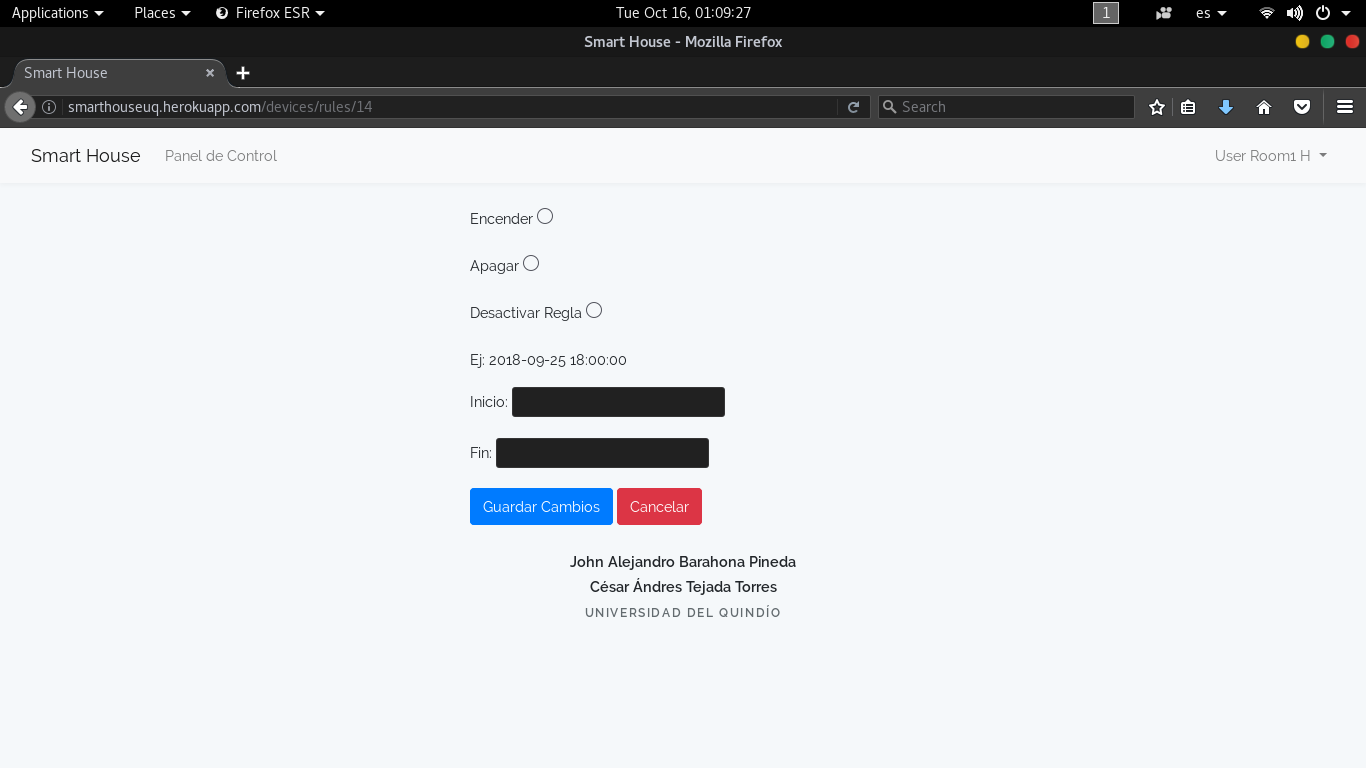
\includegraphics[width=\linewidth]{Imagenes/rules_view}
\end{wrapfigure}
Adicional a esto, si el usuario desea añadir, modificar o eliminar una regla, por ejemplo, quiere encender el bombillo led a una hora deseada, esto lo puede lograr mediante el botón de reglas en el panel de control, el cual lo redirige a la vista que se observa en la figura \ref{fig:rulesview}, en esta se indica una hora de inicio y finalización en la que el bombillo led enciende a la hora de inicio y se apaga a la hora de fin, si es la regla de apagado solo necesita una hora de inicio para apagarlo.

\end{frame}

\subsubsection{Base de Datos}
\begin{frame}
\frametitle{Resultados y Análisis}
\framesubtitle{Software | \emph{Base de Datos}}

La estructura de la base de datos se puede observar en la figura \ref{fig:db}, aquí se observan los diferentes campos que posee cada tabla, además de las llaves y sus relaciones. Las relaciones presentes en esta estructura son de tipo 1:N, es decir, por ejemplo un usuario puede tener relacionadas N casas.

\begin{figure}[H]
\centering
\caption{Base de datos SmartHouse [Imagen Propia]}
\label{fig:db}
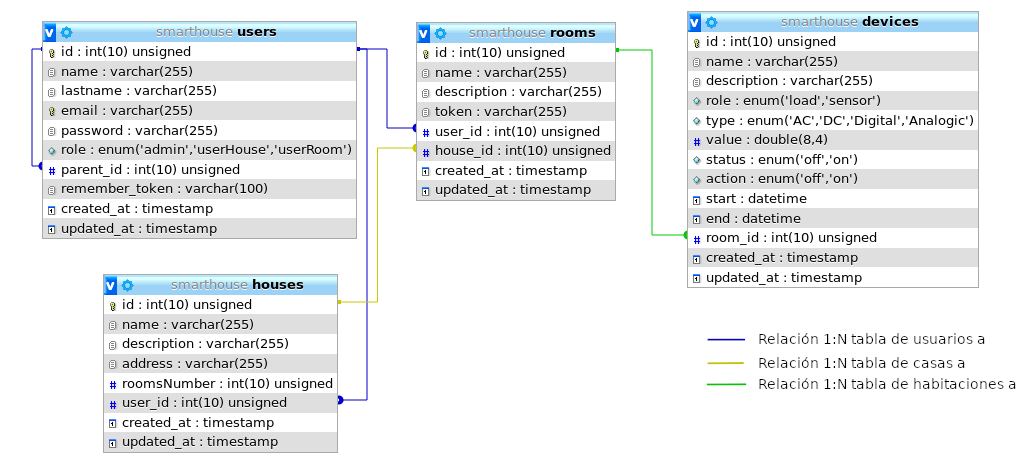
\includegraphics[width=0.75\linewidth]{Imagenes/DB}
\end{figure}

%Esta sección donde se presentan todos los resultados en cuanto al software desarrollado presenta la mayoría de funciones implementadas en este, mostrando las diversas interfaces generadas en la aplicación, cumpliendo con los requisitos de permitir el monitoreo, control y la interacción del usuario con el dispositivo presente en su habitación, por medio de diferentes items que se han evidenciado en las figuras anteriores, permitiendo cambiar el estado de las salidas y asimismo visualizar los datos producidos por los sensores. También cabe resaltar que algunas salidas tienen la posibilidad de automatizarse a través de reglas, es decir, indicarle en que momento encender o apagar cierto dispositivo que se encuentre conectado a la tarjeta como se ha mencionado.\\

%Las funcionalidades para el cambio de estado en las salidas se realizan con cuidado, generando diálogos de confirmación con el fin de que el usuario este seguro de la acción que realiza. Para ejercer control sobre la energía entrega a las cargas, se cuenta con un deslizador o slider que permite cambiar el porcentaje de esta, asimismo es significativo resaltar que todos los datos generados de la interacción del cliente con el programa, se almacenan en la base de datos enlazada a dicha aplicación permitiendo una gestión adecuada de estos. Los resultados obtenidos del diseño de este software cumplen con el objetivo a partir del cual se construye y también se tienen algunas funciones adicionales como los usuarios administradores de casa, esto asegurando la escalabilidad de la aplicación. \\
%
%En cuanto a la protección de la aplicación se han mencionado los diferentes roles que se verifican por medio del middlware presente en esta solución, pero también cabe resaltar que con el objetivo de agregar seguridad a la transacción tarjeta-servidor se usa un token, el cual es único de cada habitación y se encuentra almacenado en la tarjeta y en el servidor, como se menciona anteriormente la aplicación al recibir la petición realiza esta verificación para proceder a contestar o simplemente ignorar la petición, de acuerdo con esto se esta ofreciendo un nivel de confiabilidad en dicha comunicación.\\

\end{frame}


\subsection{Firmware}
\begin{frame}
\frametitle{Resultados y Análisis}
\framesubtitle{Firmware}
\footnotesize 
\begin{wrapfigure}{r}{0.5\linewidth}
	\centering
	\caption{Esquema de Tareas [Imagen Propia]}
	\label{fig:tareas}
	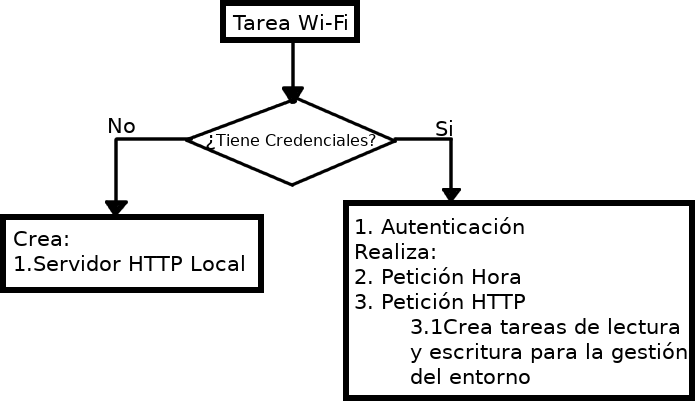
\includegraphics[width=\linewidth]{Imagenes/tareas}
\end{wrapfigure}
Como se ha mencionado anteriormente, el firmware se encuentra compuesto de tareas, en la figura \ref{fig:tareas} se observa un bosquejo del trabajo de las diferentes tareas, tomando por función principal la encargada de gestionar la conexión a Wi-Fi y almacenar sus credenciales, dependiendo del estado de si estan almacenadas o no, el sistema se comporta de una u otra forma. Si se encuentran credenciales guardadas en la tarjeta, el sistema se trata de conectar, si la conexión es exitosa comienza el proceso de actualización de la hora del sistema y también de las diferentes ordenes de la aplicación web. En cambio, si no existen credenciales el dispositivo inicia un servidor web local para que el usuario pueda proporcionarle esta información.\\

%En cada caso se crean tareas diferentes, para el suceso de no existir credenciales únicamente se configura la tarea del servidor http local, y en la otra ocurrencia se lanzan todas la demás tareas encargadas de la escritura y lectura de datos, como se menciona en las siguientes secciones. Cabe resaltar que la tarjeta tiene disponible en promedio 160KB de memoria heap con el fin de poder realizar otras operaciones o implementar más funcionalidades en esta.\\
\end{frame}

\begin{frame}[t]
\frametitle{Resultados y Análisis}
\framesubtitle{Firmware}
Se mide el promedio del tiempo en que se demora la ejecución de la tarea en dos casos, cuando realiza la primera petición después de conectado a la red, es decir, cuánto se tarda realizando las peticiones necesarias, como obtener la hora y fecha de la red y realizar la petición a la aplicación web, obteniendo una duración media de aproximadamente de 2.7s, esta depende de la disponibilidad de los diferentes servidores en la web asimismo de la velocidad y el tráfico de la red, ya que la tarjeta espera hasta que obtiene dicha hora y luego continua con la petición HTTP también esperando que el servidor responda. El otro caso es el lapso que se demora la tarea en leer los datos de los sensores, enviar la petición HTTP al servidor, recibirlos y enviarlos a los diversor actuadores, este periodo es de 1s en promedio, para conocer el dato se tomaron un total de 3056 muestras.
\end{frame}

\subsubsection{Conexión a Internet vía Wi-Fi}
\begin{frame}[t]
\frametitle{Resultados y Análisis}
\framesubtitle{Firmware | \emph{Conexión a Internet vía Wi-Fi}}
\begin{wrapfigure}{r}{0.5\linewidth}
	\centering
	\caption{Conexión a Internet vía Wi-Fi ESP32 [Imagen Propia]}
	\label{fig:conexion}
	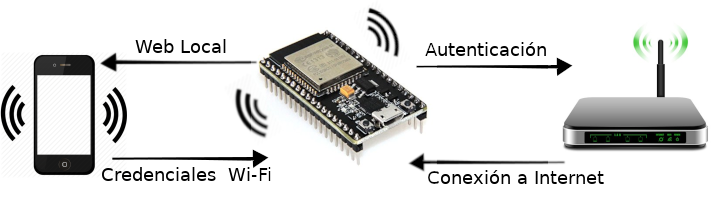
\includegraphics[width=\linewidth]{Imagenes/conexion}
\end{wrapfigure}
Los sistemas IoT deben estar conectados siempre a Internet, por tal motivo se debe brindar una forma para conectar al sistema a este, en base a esto, se desarrolla un servidor local en la tarjeta que facilitar este proceso, como se ha mencionado el módulo del ESP32 funciona como Punto de Acceso (AP) y como Cliente o Estación (STA) al mismo tiempo, aprovechando esta capacidad se usa el servidor local y se encuentra encargado de gestionar la conexión de la tarjeta vía Wi-Fi como se observa en la figura \ref{fig:conexion}.
\end{frame}


\begin{frame}[t]
\frametitle{Resultados y Análisis}
\framesubtitle{Firmware | \emph{Conexión a Internet vía Wi-Fi}}
De este modo, en la figura \ref{fig:wifi} están algunas paginas del servidor local, en la figura \ref{fig:wifi}\textbf{(a)} es posible observar la lista de las diferentes redes al alcance de la tarjeta, basta con seleccionar una red e ingresar sus credenciales para conectarse, en la figura \ref{fig:wifi}\textbf{(b)} se observan los detalles de la conexión actual y también la opción de desconectarse. Su funcionamiento es muy intuitivo, se selecciona la red a la que se desea conectar la tarjeta, se ingresan sus credenciales y posteriormente el dispositivo verifica si la conexión fue exitosa o no; si lo es, la tarjeta esta lista para su funcionamiento, no obstante, se debe reiniciar para que solo quede funcionando como STA y no en el modo dual, además de esto si las credenciales de la red cambian, se incluye un botón para el borrado de estas, con el fin de que se puede configurar de nuevo el enlace con la red Wi-Fi.

\end{frame}

\begin{frame}[t]
\frametitle{Resultados y Análisis}
\framesubtitle{Firmware | \emph{Conexión a Internet vía Wi-Fi}}

\begin{figure}[H]
	\centering
	\caption{Aplicación Conexión a Wi-Fi [Imagen Propia]}
	\label{fig:wifi}
	\subfigure[Lista de Redes]{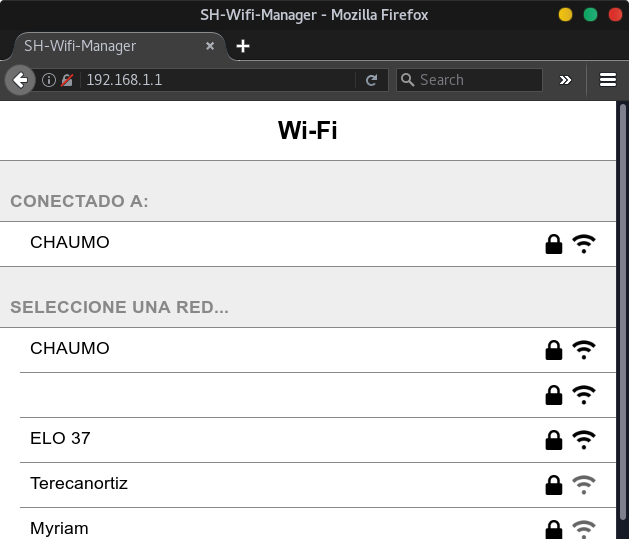
\includegraphics[width=0.45\linewidth]{Imagenes/w_status}
		\label{fig:red}}
	\subfigure[Datos de Conexión]{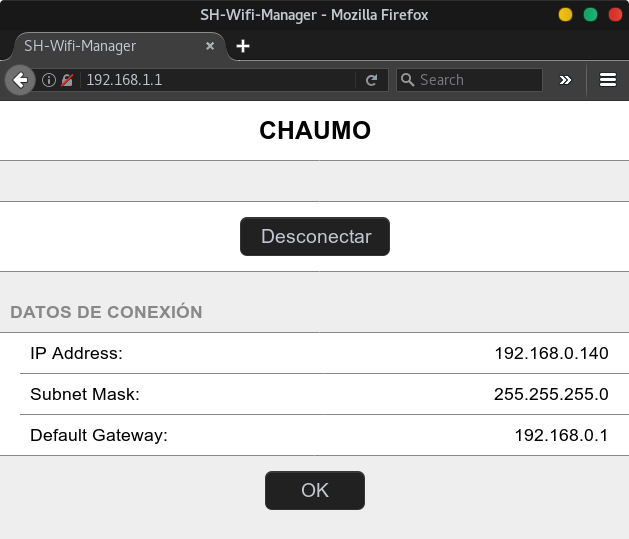
\includegraphics[width=0.45\linewidth]{Imagenes/w_red}
		\label{fig:opt}}
\end{figure}

\end{frame}

\subsubsection{Escritura de Datos en la Aplicación Web}
\begin{frame}[t]
\frametitle{Resultados y Análisis}
\framesubtitle{Firmware | \emph{Escritura de Datos en la Aplicación Web}}
\footnotesize
\begin{wrapfigure}{r}{0.5\linewidth}
	\centering
	\caption{URL de la petición HTTP [Imagen Propia]}
	\label{fig:json}
	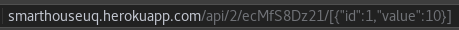
\includegraphics[width=\linewidth]{Imagenes/JSON}
\end{wrapfigure}
Los datos que lee la tarjeta provienen de los diferentes sensores que tiene conectados según se ha mencionado, se usan diversos tipos, de estado para sensar la presencia, de calidad de aire entre otros presentes en esta. Para la escritura de los datos en el firmware se desarrollan varias tareas encargadas de leerlos y enviarlos a una tarea central. Los datos que están enviando contienen el id del dispositivo y la medida que lee en ese momento, estos se envían en forma de texto en formato JSON, de este modo, la tarea central los gestiona y envía a la aplicación con el mismo formato, organizandolos en la petición HTTP tipo GET que realiza, así la url que la tarjeta solicita, incluyendo el JSON de cada sensor, se observa en la figura \ref{fig:json}, de esta manera, en la url se encuentra el dominio del servidor, y la dirección que contiene el id y token de la habitación, por último se halla la información del sensor en formato JSON, que se compone por el id y el valor de este. La aplicación ya se encarga de almacenarlos y mostrarlos al usuario como se menciona anteriormente.

\end{frame}

\subsubsection{Lectura de Datos de Internet}
\begin{frame}[t]
\frametitle{Resultados y Análisis}
\framesubtitle{Firmware | \emph{Lectura de Datos de Internet}}
Para la configuración y comparación de las reglas que suministra el usuario a el dispositivo que desee controlar, es necesario contar con la hora actual y que se siga actualizando localmente gracias al RTC que posee internamente el ESP32, así, al inicio de la aplicación, se sincroniza y almacena la hora actual de la red, por medio del protocolo SNTP. Estas reglas actúan en cuanto a que encienda o apague un dispositivo en un instante dado, después de obtener este dato la ejecución programa continua con normalidad para realizar las diferentes peticiones a la aplicación web.
\end{frame}

\begin{frame}[t]
\frametitle{Resultados y Análisis}
\framesubtitle{Firmware | \emph{Lectura de Datos de Internet}}

\begin{wrapfigure}{r}{0.5\linewidth}
	\centering
	\caption{Respuesta de la APP Web a la Tarjeta [Imagen Propia]}
	\label{fig:httprqstesp}
	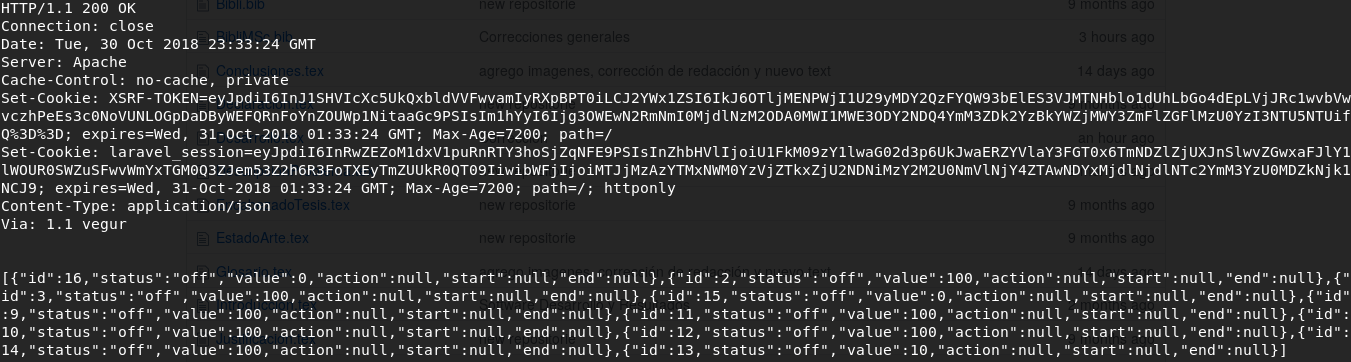
\includegraphics[width=\linewidth]{Imagenes/HTTPRqstesp}
\end{wrapfigure}
La interacción del usuario se da con la aplicación web mencionada anteriormente, de este modo la tarjeta siempre se debe actualizar, para esto, cuando la tarjeta envía los datos de los sensores, la aplicación responde con datos de cabecera HTTP y además la información de los dispositivos que controla la tarjeta, esta los recibe en una cadena texto en formato JSON como se observa en la figura \ref{fig:httprqstesp}, los procesa y los dirige a las tareas pertinentes ya sea para encender o apagar algún dispositivo conectado a la tarjeta, también remite las reglas que el usuario ha definido.

\end{frame}

%Según lo presentado en esta sección, la tarjeta cuenta con funcionalidades para conectarse con internet por medio de wi-fi, toda la configuración del cómo hacerlo la realiza el usuario mediante las herramientas ofrecidas por el programador, es decir, el servidor local. Durante el desarrollo de este programa se comprenden diferentes funciones que provee un RTOS, de manera que es viable haber desarrollado esta aplicación basado en este sistema operativo.\\

%Analizando los tiempos de resolución de la petición http, siempre se tiene una media de 1s el cual es un tiempo de respuesta aceptable dadas todas las funcionalidades provistas en el programa, aunque este tiempo varia, ya que el haber utilizado el puerto serie para observar estos resultados, esta comunicación agrega también tiempo al procesamiento, así que es un aproximado, ya que asimismo interfiere la velocidad en la conexión a internet y la señal de recepción de wi-fi.\\

%Por los resultados expuestos, el programa esta realizando correctamente las funciones necesarias para el monitoreo y control del ambiente de instalación, es decir, se cumple con los alcances provistos y además aún existen recursos de procesamiento para agregar nuevas funcionalidades o mejorar el desempeño.

\subsection{Hardware}
\begin{frame}[t]
\frametitle{Resultados y Análisis}
\framesubtitle{Hardware}
\small
\begin{wrapfigure}{r}{0.5\linewidth}
	\centering
	\caption{Tarjeta SmartHouse [Imagen Propia]}
	\label{fig:tarjeta}
	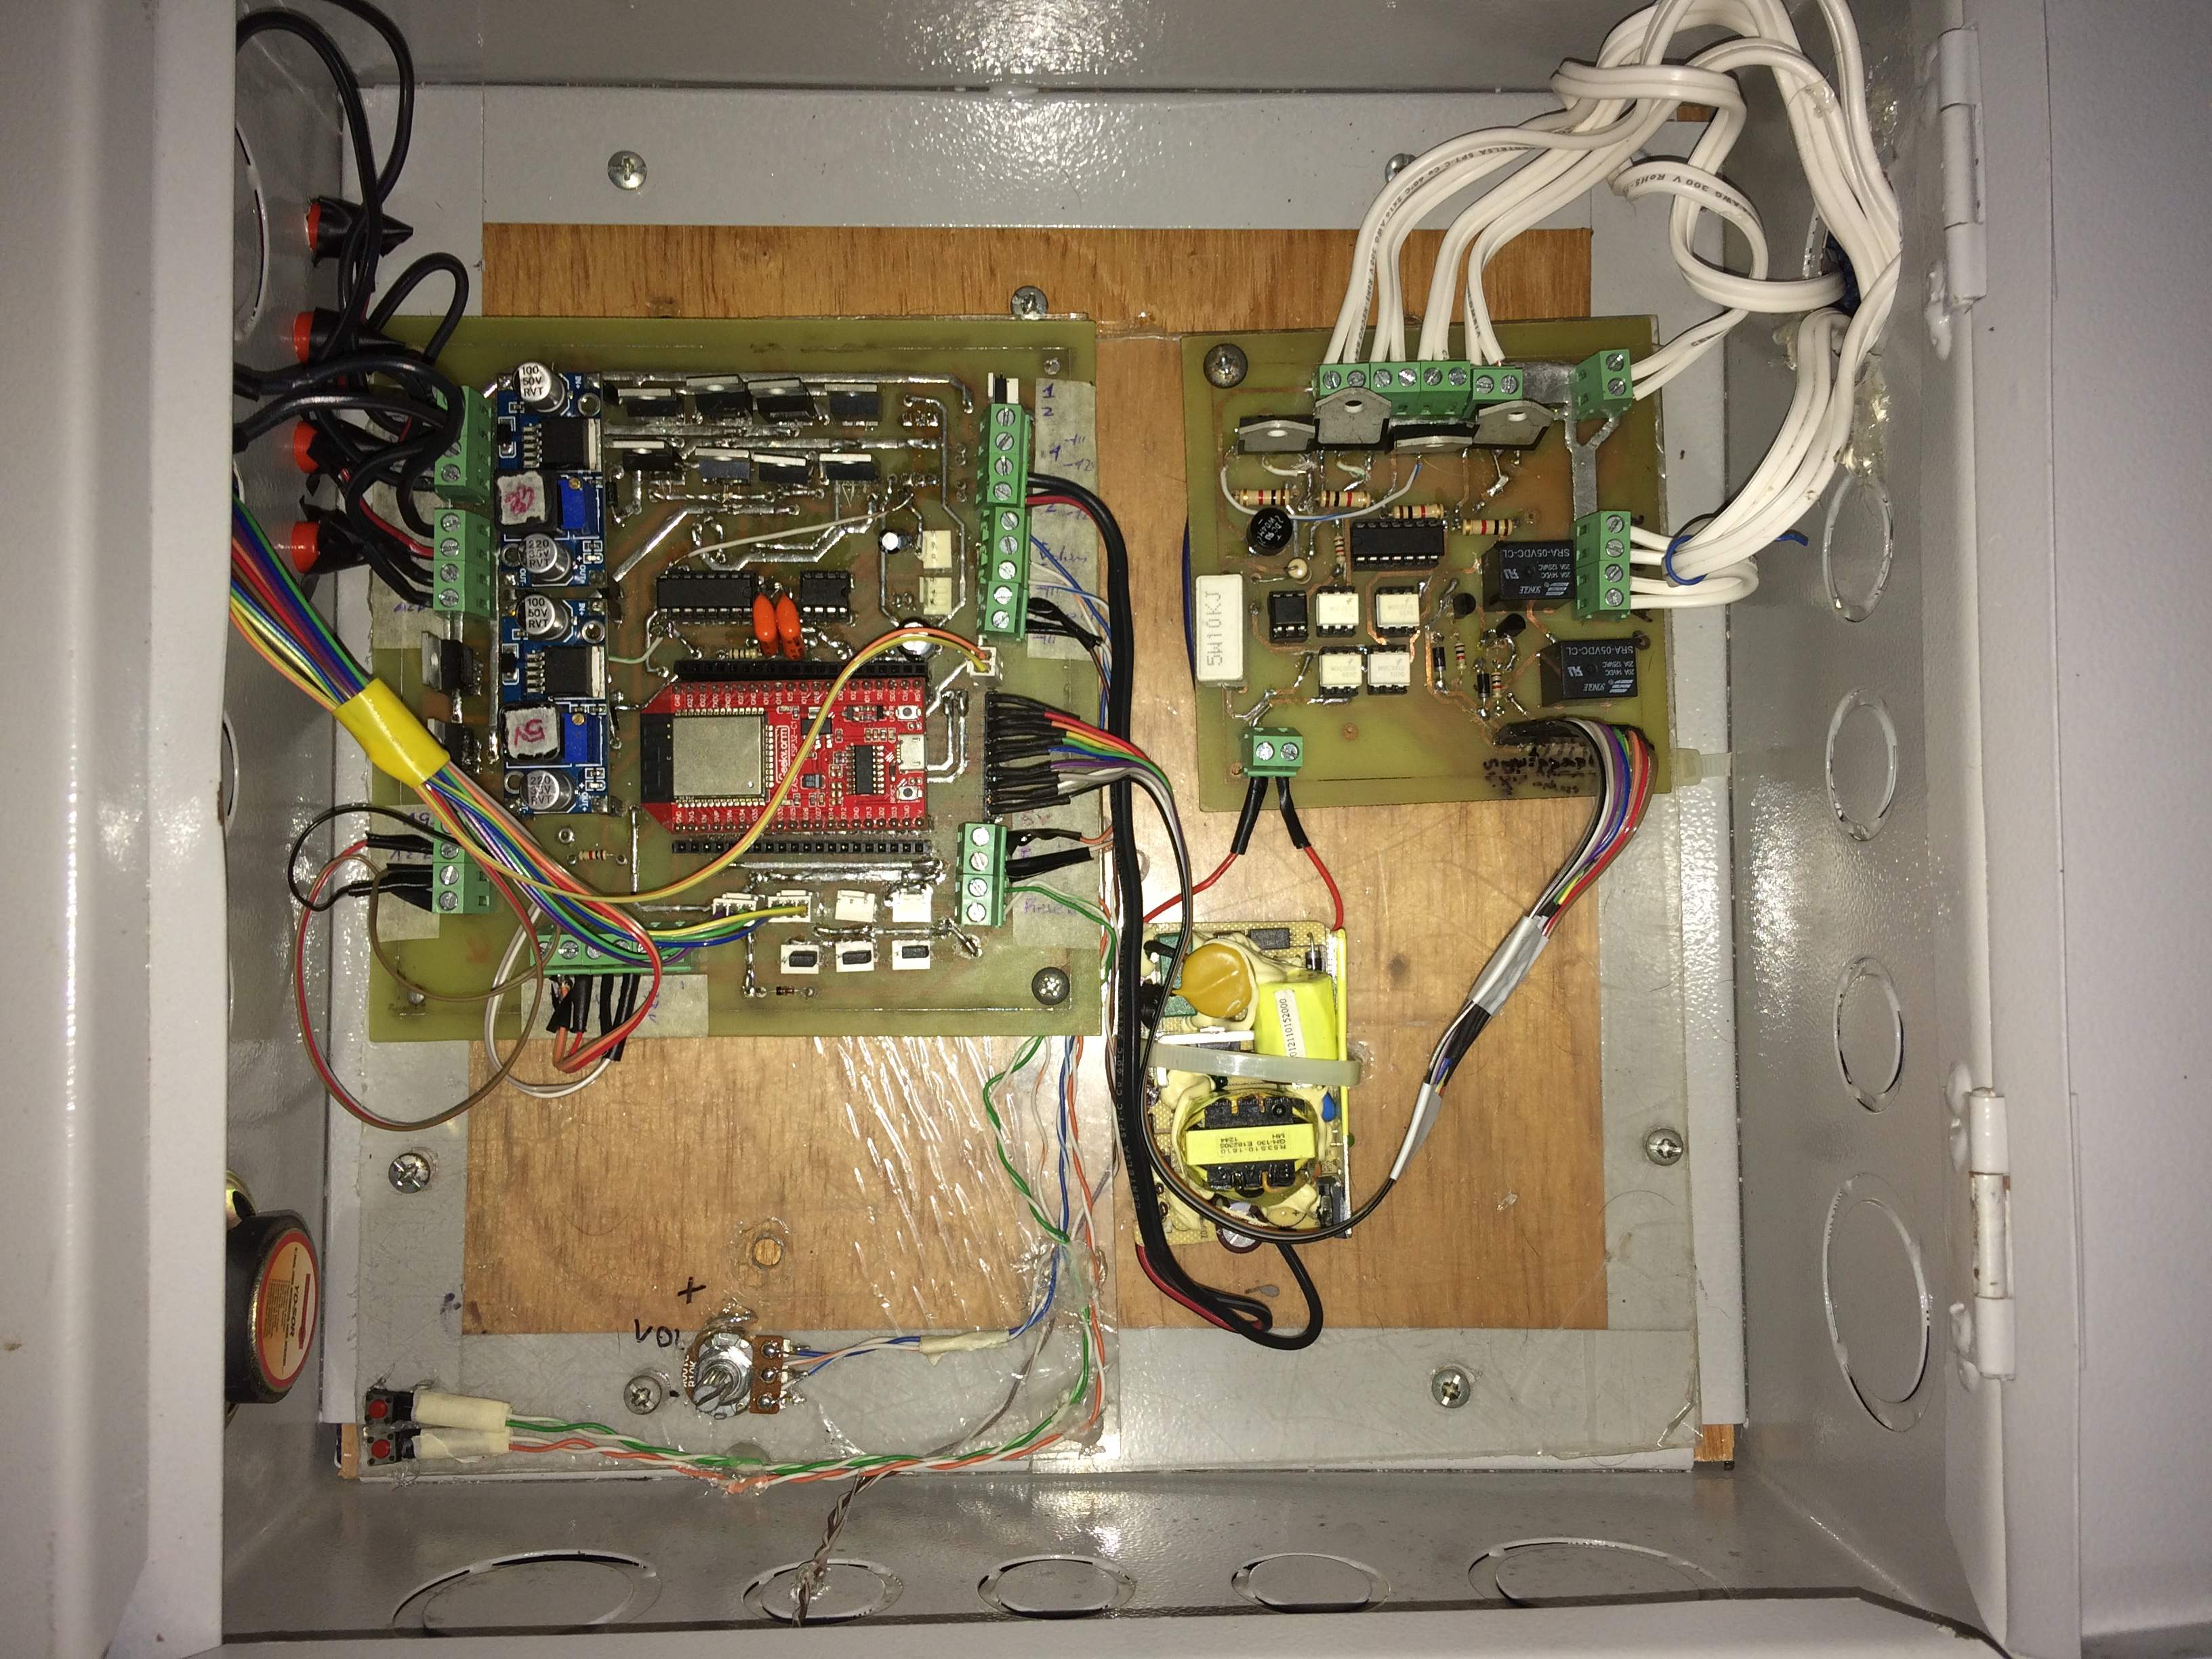
\includegraphics[width=\linewidth]{Imagenes/Tarjeta}
\end{wrapfigure}
De acuerdo con los circuitos diseñados en la sección donde se propone el desarrollo de hardware de la solución IoT, en la figura \ref{fig:tarjeta} se observan las diferentes tarjetas ya ensambladas en una caja eléctrica para probar el funcionamiento del prototipo. Las salidas y entradas están distribuidas según lo propuesto, para las salidas AC se usan toma corrientes para conectar allí los diversos dispositivos, para las salidas DC se utilizan conectores hembra tipo banana para facilitar la conexión de estos dispositivos.
\end{frame}

\begin{frame}[t]
\frametitle{Resultados y Análisis}
\framesubtitle{Hardware}
\small
\begin{wrapfigure}{r}{0.75\linewidth}
	\centering
	\caption{Descripción caja eléctrica tarjeta SmartHouse [Imagen Propia]}
	\label{fig:labels}
	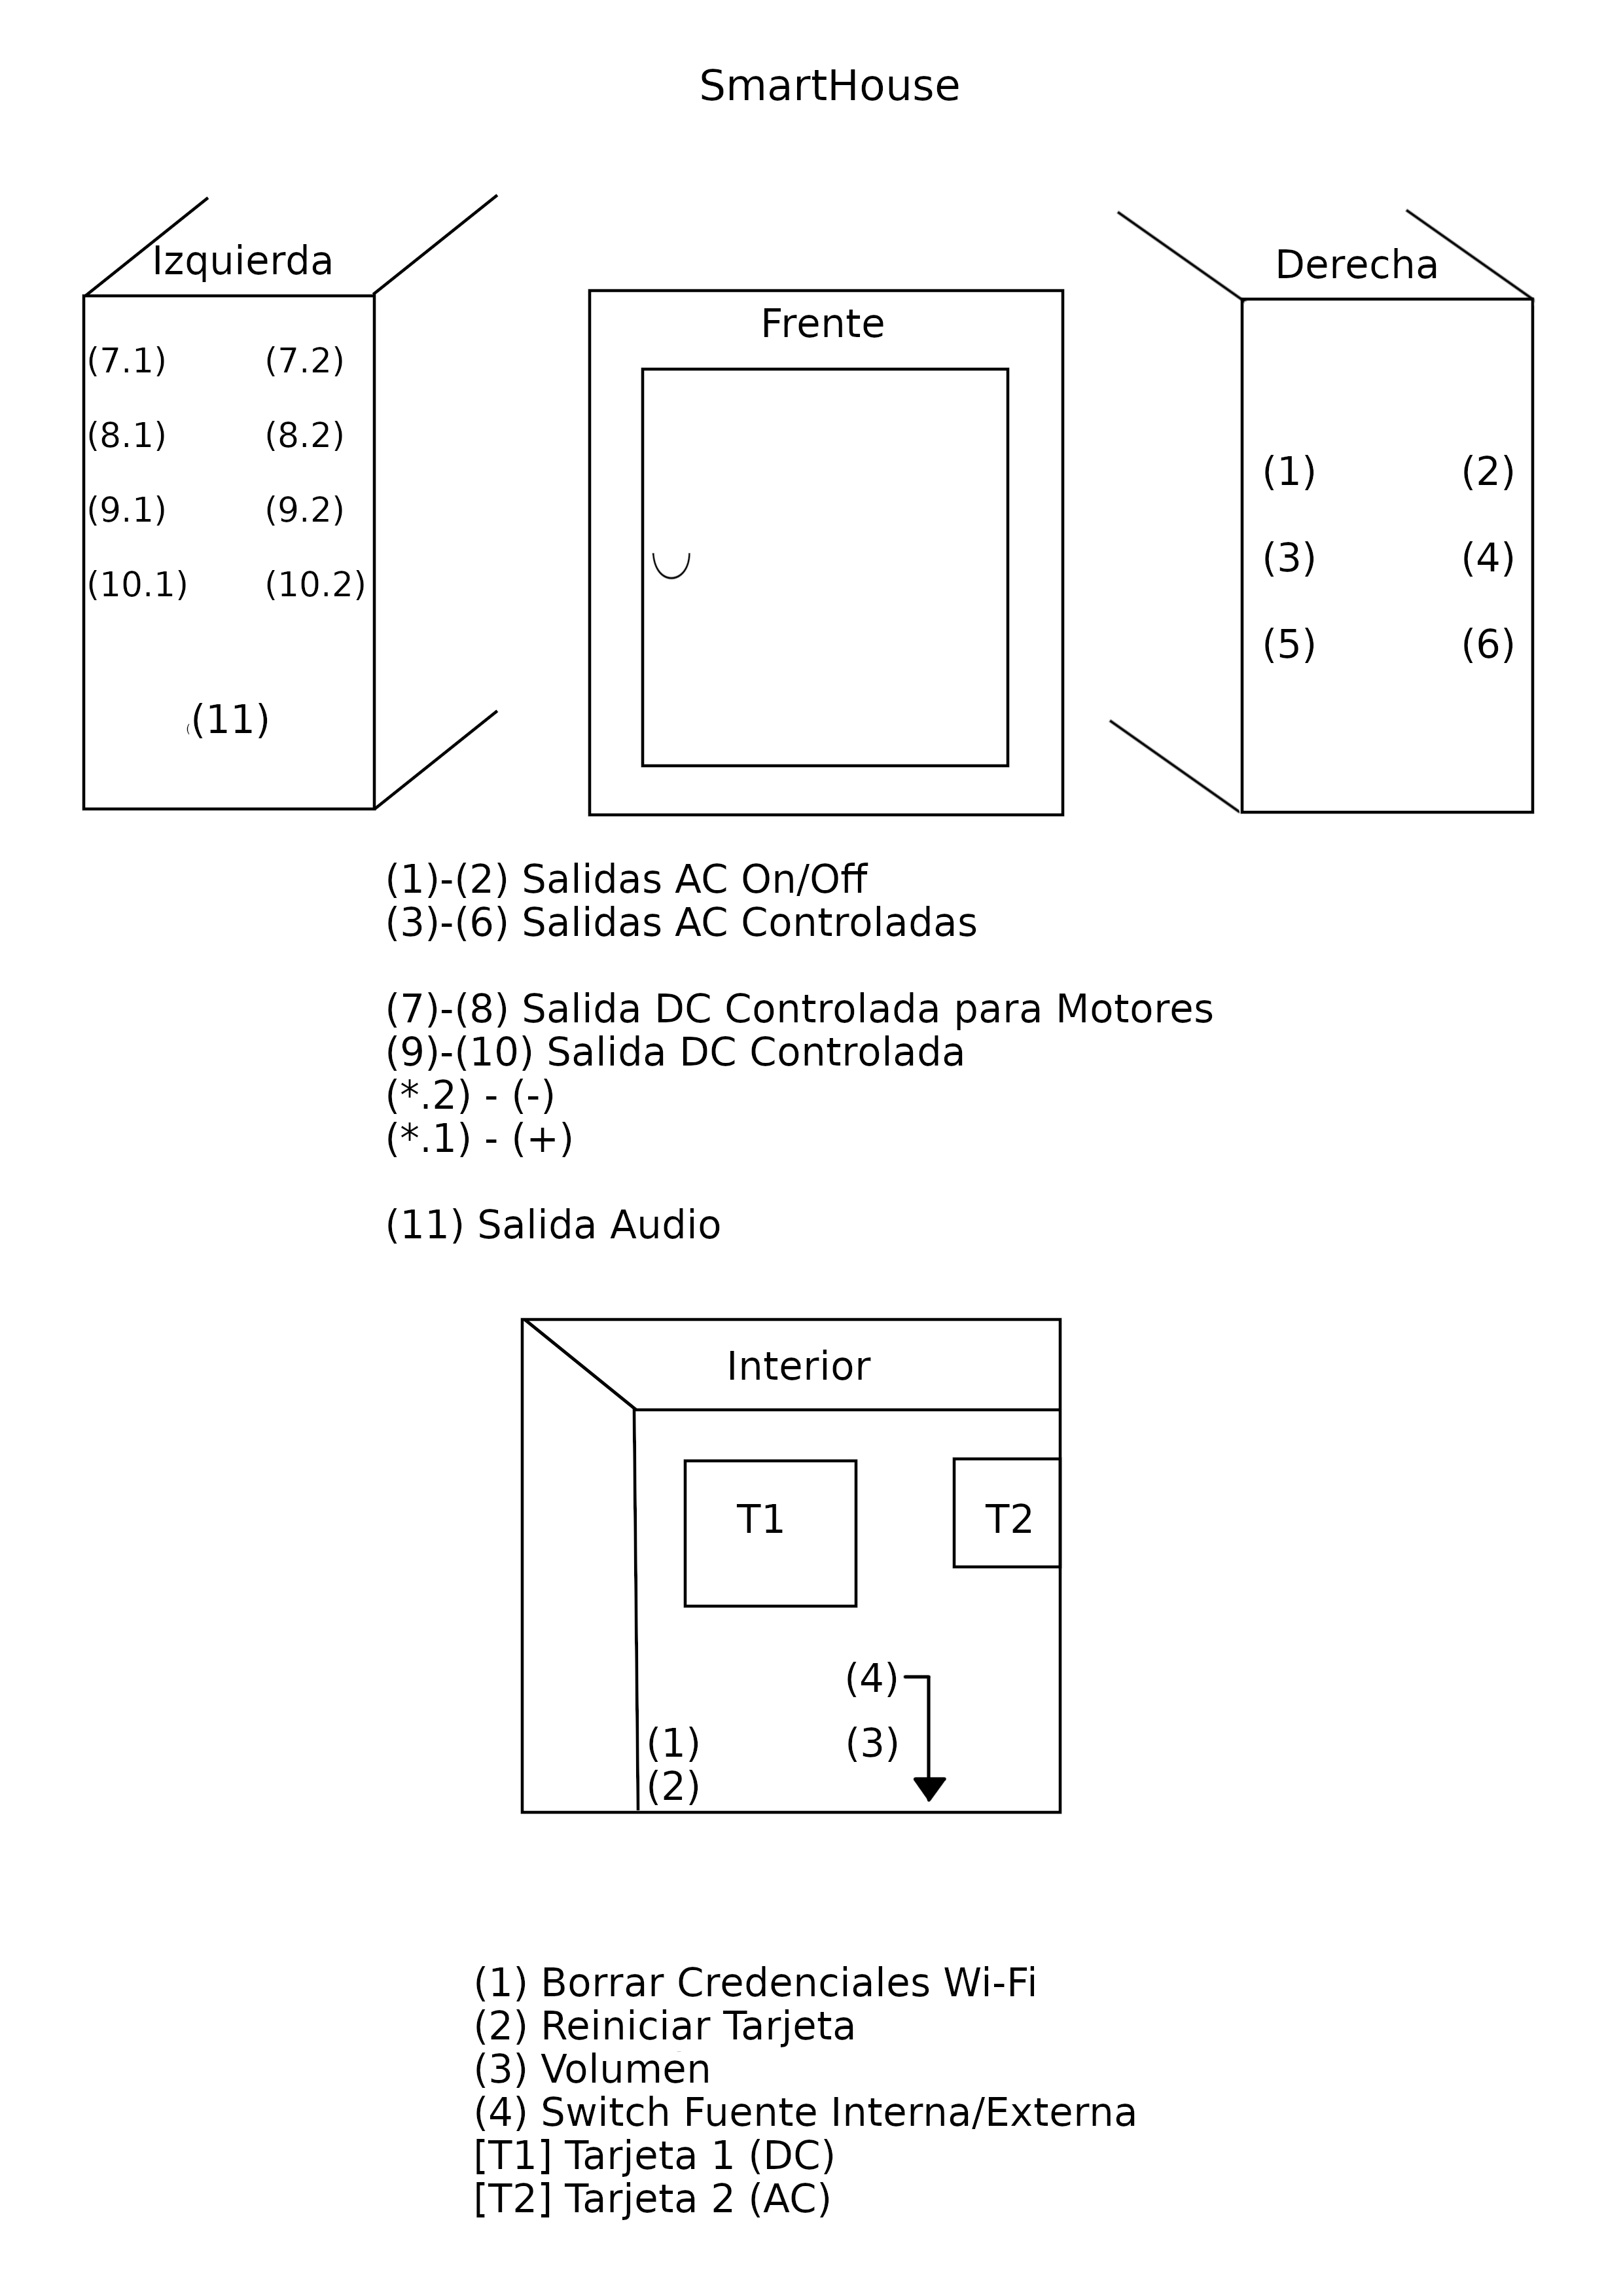
\includegraphics[width=0.47\linewidth]{Imagenes/labels}
\end{wrapfigure}
La distribución de las diferentes salidas que posee la tarjeta se organizo en pegatinas y se colocaron sobre la caja eléctrica, la figura \ref{fig:labels} muestra esta información, tanto para la parte interna como externa de la caja.
\end{frame}

\begin{frame}[t]
\frametitle{Resultados y Análisis}
\framesubtitle{Hardware}
\small
\begin{wrapfigure}{r}{0.5\linewidth}
	\centering
	\caption{Control de potencia AC por ángulo de fase [Imagen Propia]}
	\label{fig:ACc}
	\subfigure[Potencia al 100\%]{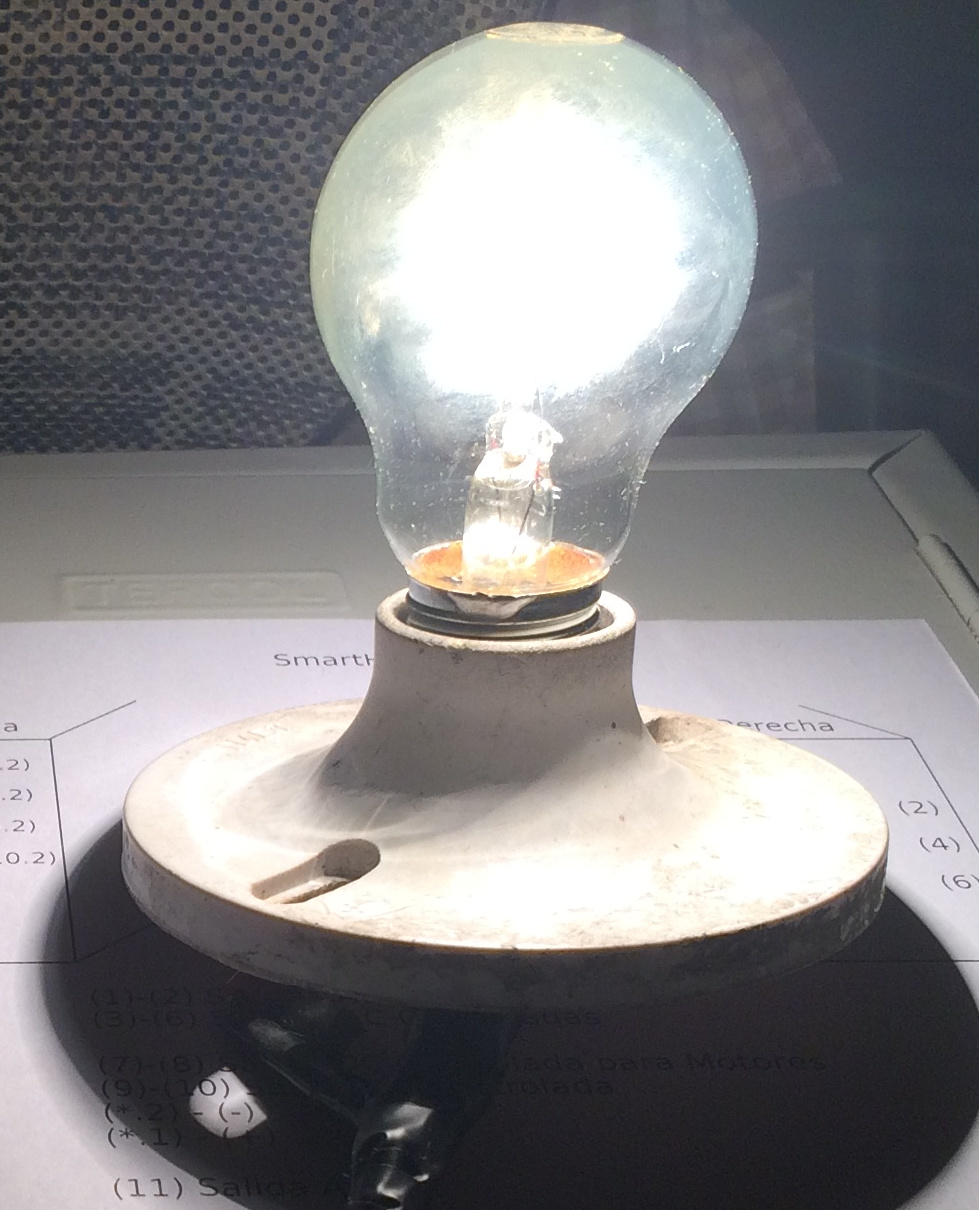
\includegraphics[width=0.45\linewidth]{Imagenes/AC1}}
	\subfigure[Potencia al 20\%]{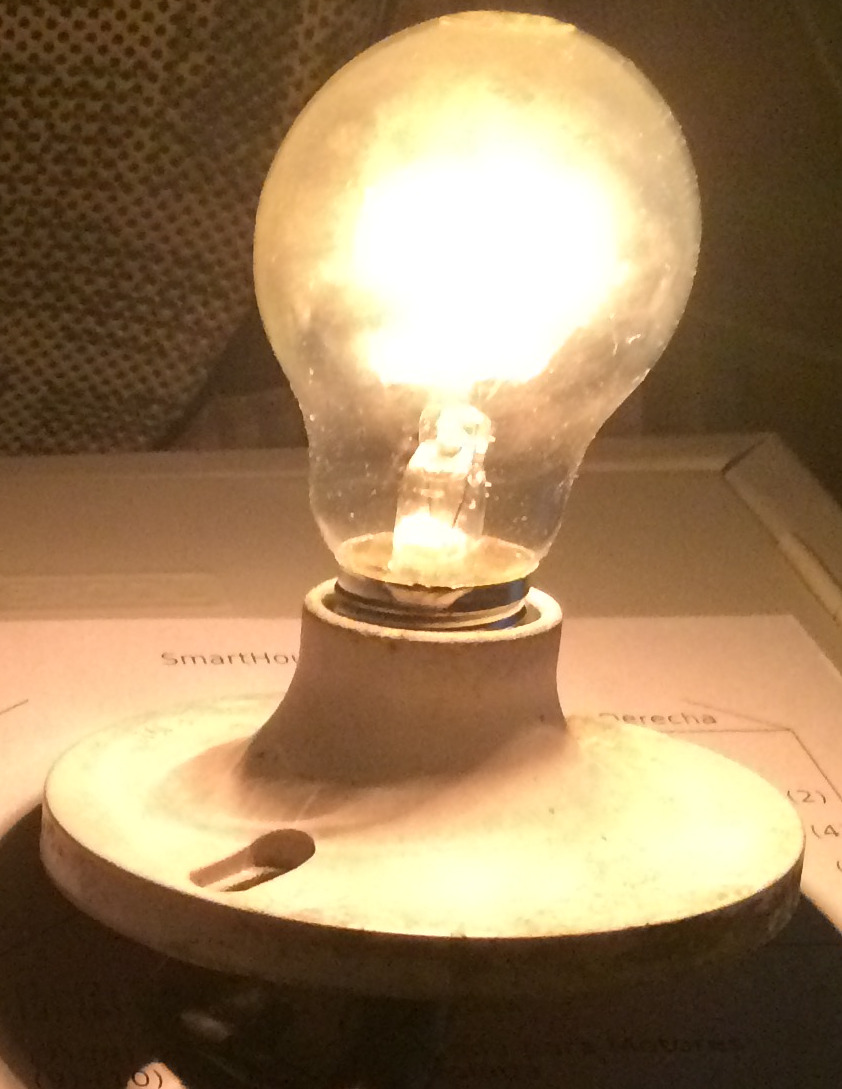
\includegraphics[width=0.43\linewidth]{Imagenes/AC0}}
\end{wrapfigure}
Conforme a lo mencionado anteriormente, el sistema se ha probado con cargas AC como bombillos LED entre 7W y 20W, de filamento de 100W, probando funcionalidades como el control de potencia AC por ángulo de fase, obteniendo los resultados esperados, según se observa en la figura \ref{fig:ACc}\textbf{(a)} donde la carga tiene el 100\% de la potencia y en la figura \ref{fig:ACc}\textbf{(b)} con el 20\% de esta. El voltaje de alimentación viene dado por la red eléctrica, la tarjeta simplemente conmuta el estado de la alimentación o controla la potencia entregada. 

\end{frame}


\begin{frame}[t]
\frametitle{Resultados y Análisis}
\framesubtitle{Hardware}
\begin{wrapfigure}{r}{0.5\linewidth}
	\centering
	\caption{Control de Cargas DC [Imagen Propia]}
	\label{fig:DCc}
	\subfigure[Potencia al 100\%]{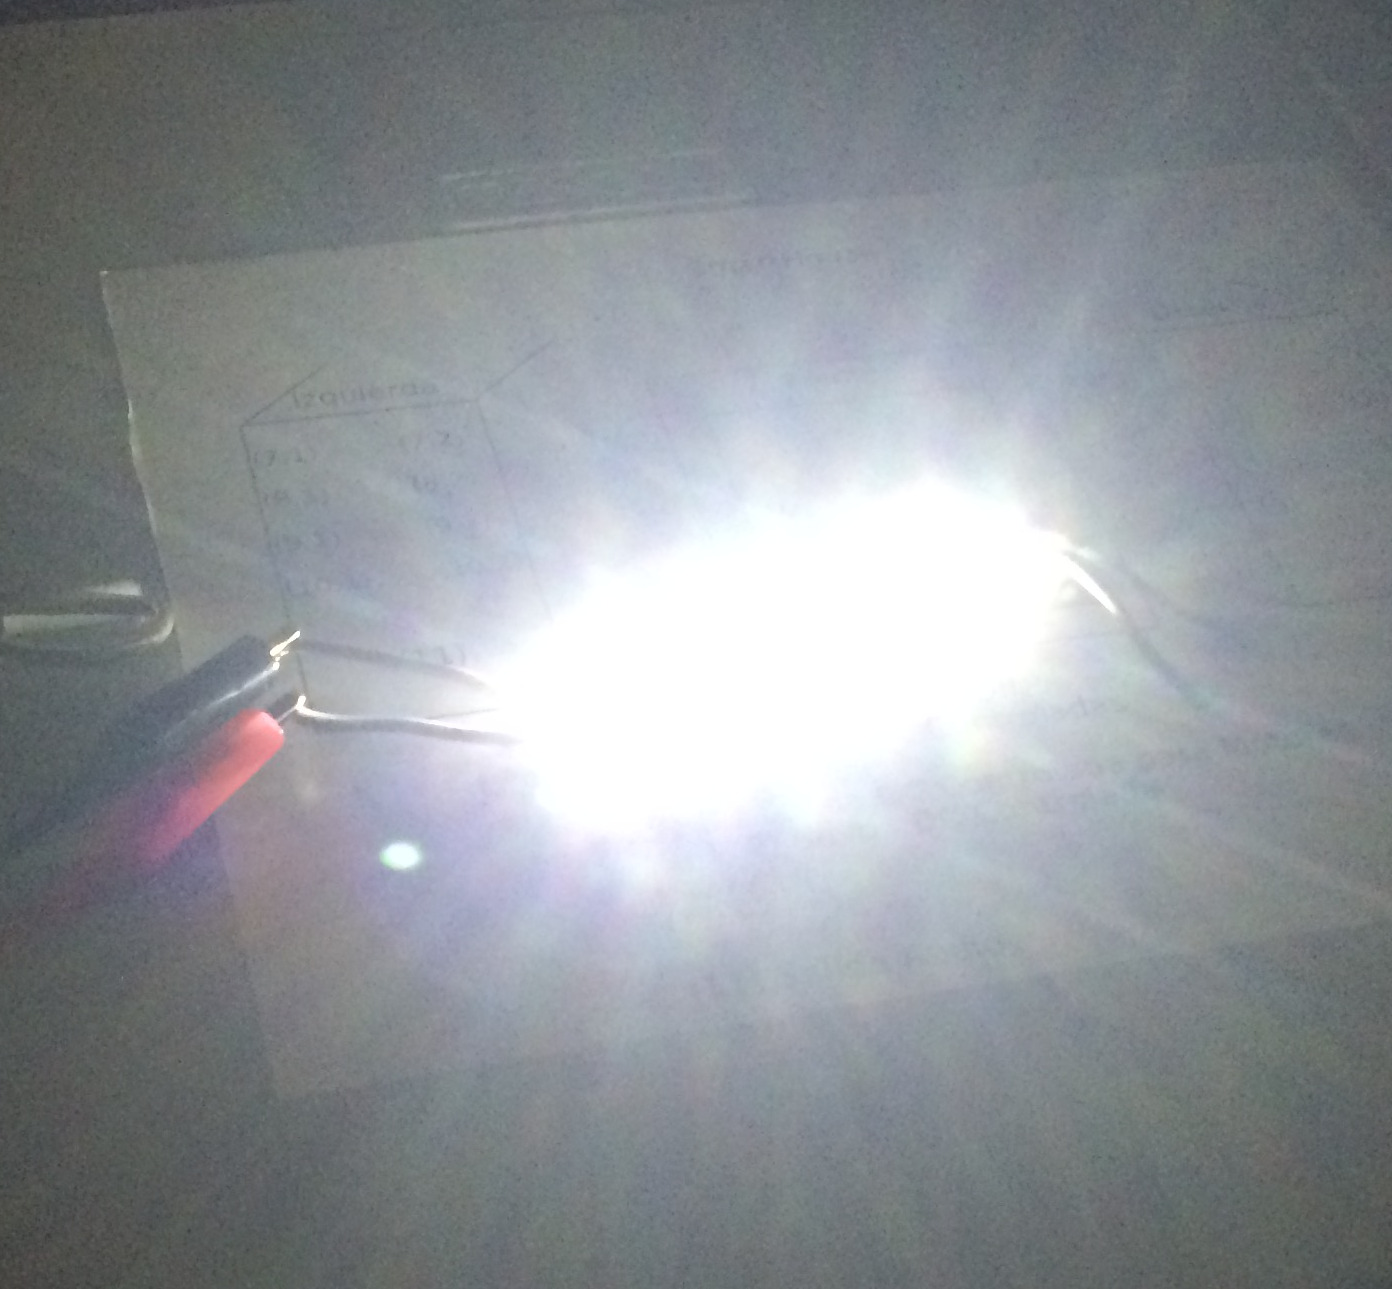
\includegraphics[width=0.45\linewidth]{Imagenes/DC1}}
	\subfigure[Potencial al 10\%]{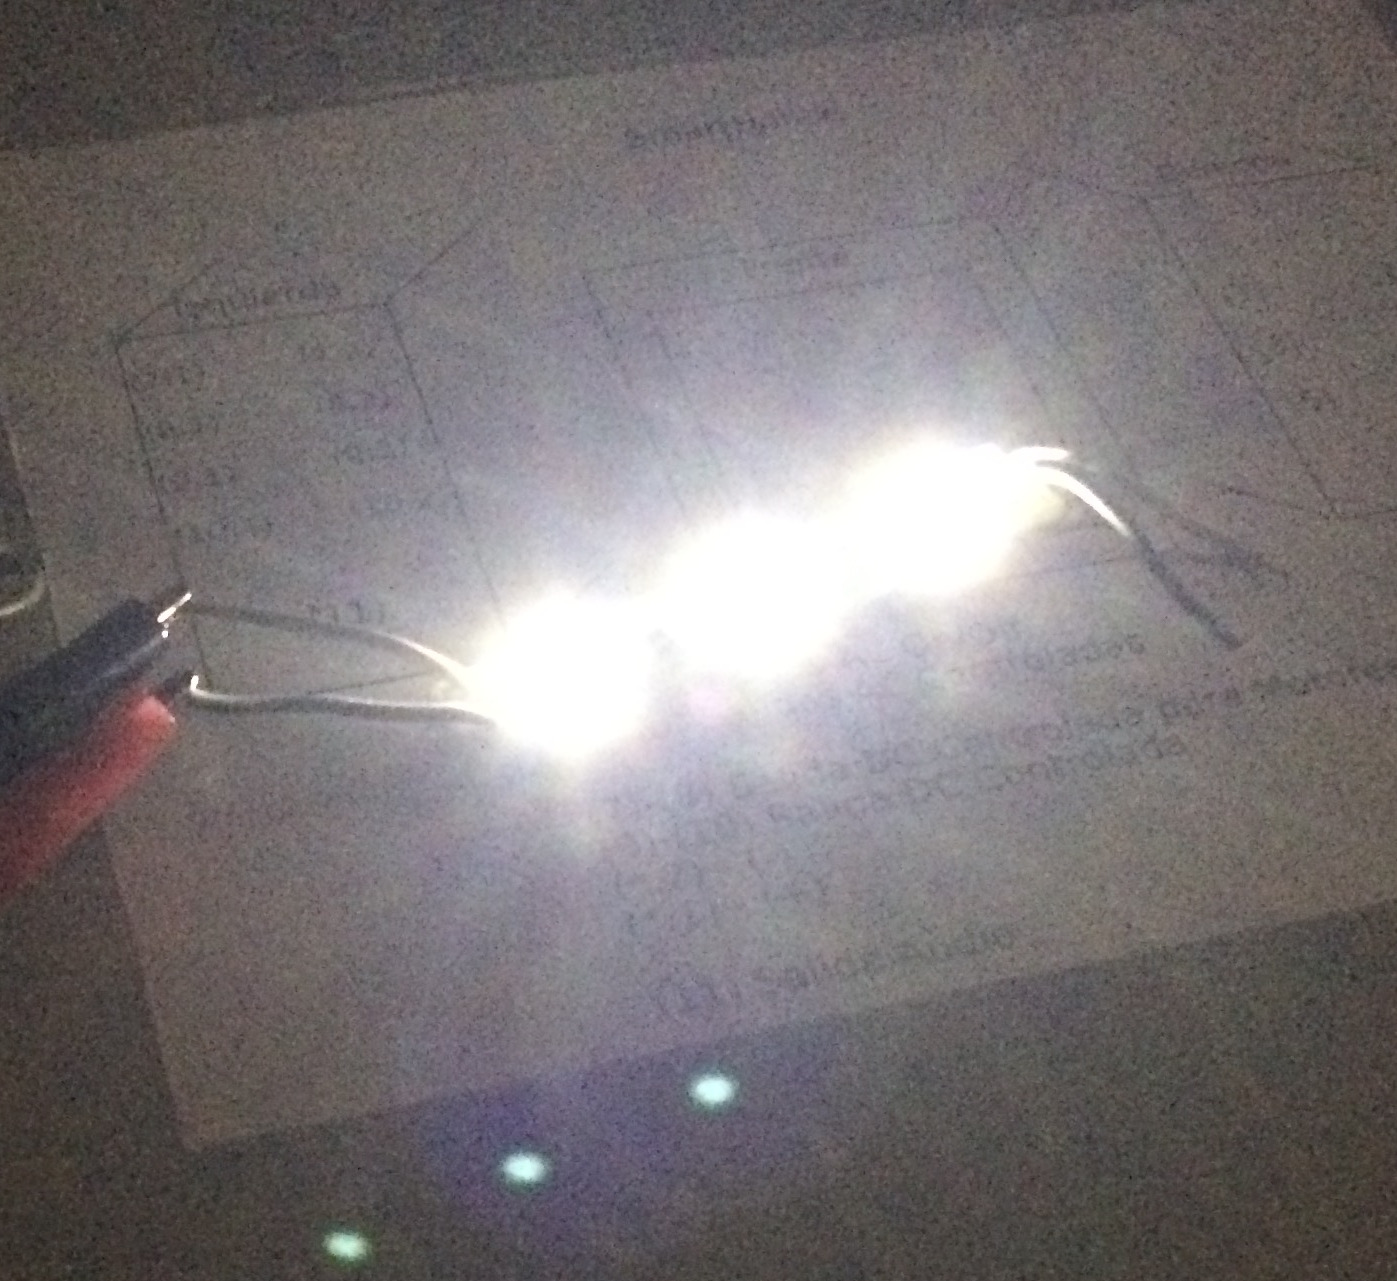
\includegraphics[width=0.455\linewidth]{Imagenes/DC0}}
\end{wrapfigure}
Para las salidas DC se realizan pruebas con un motor DC de 1W, además de una tira LED de 1W, la cual se le varia la energía entrega, como se observa en la figura \ref{fig:DCc}\textbf{(a)} la carga tiene el 100\% de la energía y en la figura \ref{fig:DCc}\textbf{(b)} solamente el 10\%. Estas cargas se alimentan con 12VDC directamente desde la fuente o convertidor AC-DC, los circuitos que se implementan simplemente conmutan el estado de encendido/apagado o por medio de PWM variar la energía entregada.

\end{frame}



%En esta sección se evidencia tanto el hardware implementado, como su correcto funcionamiento de acuerdo con los requisitos propuestos, proporcionando las diferentes funcionalidades para que el firmware realice la gestión adecuada, es decir, controlar las salidas y recibir la información de los entradas. Se han construido diferentes circuitos, los cuales por medio del programa gestiona los diferentes dispositivos conectados a este.\\

%Se observa que el hardware quedo dividido en dos tarjetas, esto para facilitar la construcción y distribución de los diferentes elementos utilizados, si se usan componentes superficiales y se aumentan las capas de la tarjeta es posible reducir el tamaño y hasta integrarlas en una sola board. En la construcción de estas tarjetas se comprende diferentes funcionamientos en cuanto a los triac y los transistores mosfet, reforzando conocimientos que se habían adquirido.\\

\subsection{Prueba Beta Cerrada}

\begin{frame}[t]
\frametitle{Resultados y Análisis}
\framesubtitle{Prueba Beta Cerrada}
Para la prueba beta se escoge un grupo de personas, las cuales interactuan directamente con la aplicación web y el prototipo de la tarjeta SmartHouse, se detallan los diferentes items a evaluar mencionados anteriormente, como el ingreso a la aplicación, visualización de los datos almacenados en esta y el control de los dispositivos.\newline

Así, para evaluar estas características se formulan las siguientes preguntas, que se califican de acuerdo con una escala tipo likert \cite{lik} de uno a cinco en la cual, cinco es la calificación máxima y uno la mínima. Estas se formulan para evidenciar la postura del cliente en cuanto a las funcionalidades de la aplicación.\\
\end{frame}

\begin{frame}[t]
\frametitle{Resultados y Análisis}
\framesubtitle{Prueba Beta Cerrada}
\footnotesize
La prueba se realiza a quince personas, entre los cuales algunos son estudiantes de ingería electrónica y personas ajenas a este tipo de escenarios, los resultados de la prueba se consignan en la tabla \ref{table:enc}.

\begin{table}[H]
	\begin{center}
		\caption{Resultados por pregunta.}
		\label{table:enc}
		\begin{tabular}{|c|c|}
			\hline 
			\textbf{Número de la Pregunta} & \textbf{Promedio} \\ 
			\hline 
			1 & 4.5\\ 
			\hline 
			2 & 4.8\\ 
			\hline 
			3 & 4.5\\ 
			\hline 
			4 & 5.0\\ 
			\hline 
			5 & 4.9\\ 
			\hline 
			6 & 4.9\\ 
			\hline 
			7 & 4.3\\ 
			\hline 
			8 & 4.3\\ 
			\hline 
			9 & 4.8\\ 
			\hline 
			\textbf{Total} & \textbf{4.7}\\ 
			\hline 
		\end{tabular} 
	\end{center}
\end{table}

\end{frame}


\begin{frame}[t]
\frametitle{Resultados y Análisis}
\framesubtitle{Prueba Beta Cerrada}
\small
De acuerdo con los resultados es necesario analizar cada pregunta individualmente y también en su totalidad, así se pueden identificar las funciones a mejorar en el sistema. Con respecto al método de conexión de la tarjeta a Internet se obtiene un promedio de 4.5, indicando que los pasos que se deben cumplir para realizarlo están claros pero aún falta mejorar, esto sucede por la poca interacción que el usuario normalmente tiene con la configuración de dispositivos, de este modo se puede brindar ayuda telefónica o del servicio técnico en momento de la instalación.\newline

Asimismo, la interfaz que se provee para realizar la conexión del sistema a la red Wi-Fi obtiene una calificación de 4.8, exponiendo que es de fácil uso pero faltan explicaciones en cuanto al momento de ingresar a esta, ya que se puede implementar también un DNS con la finalidad de que los usuarios no ingresen una dirección IP al navegador sino que escriban un nombre de dominio.\\
\end{frame}

\begin{frame}[t]
\frametitle{Resultados y Análisis}
\framesubtitle{Prueba Beta Cerrada}
Además, em caso de que la red Wi-Fi cambie sus credenciales se provee un pulsador para eliminar estas, esta funcionalidad recibe una calificación de 4.5, algunos de los comentarios realizados sugieren el cambio de posición de este botón, ya que no se visualiza fácilmente y de una explicación un poco más detallada de esto, si es posible tener acompañamiento del personal técnico.\newline

Después, al ingresar a la pagina web se presentan de manera clara los botones en la interfaz, es decir, el inicio de sesión obtiene una calificación de 5.0 lo que indica que para el usuario es fácil realizar dichas acciones, ya que los usuarios normalmente están muy familiarizados con estas, por ejemplo, cuando ingresan a redes sociales.\\
\end{frame}

\begin{frame}[t]
\frametitle{Resultados y Análisis}
\framesubtitle{Prueba Beta Cerrada}

En cuanto a cómo se presenta la información de los diferentes dispositivos en el panel de control se obtiene 4.9, es decir, estos datos se presentan de manera clara y entendible para el usuario pero falta añadir un poco de explicación con el fin de que este se familiarice más con la interfaz propuesta.\newline

Luego, en la parte de gestionar las salidas desde la web la calificación fue de 4.9, por lo tanto la manera en que se encienden, apagan y se controlan los diferentes dispositivos es claro, pero por ejemplo, por el tiempo de recarga automática de la página a veces es necesario cierta rapidez para cambiar alguna característica. Por tal motivo se modifica este lapso de 10s a 20s, de acuerdo con las observaciones realizadas.\\

\end{frame}

\begin{frame}[t]
\frametitle{Resultados y Análisis}
\framesubtitle{Prueba Beta Cerrada}
\small
Por otra parte, el tiempo de respuesta después de gestionar un dispositivo en la aplicación obtuvo 4.3, es una calificación baja respecto a las demás, este resultado depende de diversas circunstancias que se presenten durante la realización de la instrucción y todo lo que esto acarrea, desde el momento en que el usuario realiza la acción, es decir, que no coincida con la actualización automática de la pagina, la rapidez del navegador que posee el dispositivo desde el que realizan la actividad, entre otros factores también propios del programa, por ejemplo, el tiempo que la tarea esta suspendida o el lapso de ejecución de la instrucciones.\newline

Respecto a la activación de las reglas para los dispositivos la calificación es de 4.3, ya que no es muy claro para el usuario qué es una regla dentro de la aplicación, además de que no están disponibles en todas las salidas por este motivo se puede mejorar la interfaz con el fin de definirlas de una mejor manera, asimismo hacerla más interactiva e intuitiva con el cliente.\\

\end{frame}

\begin{frame}[t]
\frametitle{Resultados y Análisis}
\framesubtitle{Prueba Beta Cerrada}
\small
Además, en una escenario general la facilidad de uso de la aplicación web recibe 4.8 como calificación, es decir que cumple con las expectativas, pero requiere agregar ciertos cambios para que sea más fácil de usar la primera vez que el cliente tiene contacto con esta. En este punto se resaltan observaciones ya mencionadas como el tiempo de actualización automática de la aplicación y la distribución del panel de control.\newline

En resumen, la aplicación recibe una calificación de 4.7, por lo tanto se puede decir que las funcionalidades requeridas están programadas de una manera adecuada y simple para que el usuario disponga de ellas, pero es posible mejorarlas con el objetivo de que sean mucho más intuitivas para el usuario y que no se le presenten dudas al momento de usarla. Conforme a las observaciones obtenidas durante la prueba se han modificado algunas partes del sistema, que no tienen un impacto significativo sobre los objetivos ni alcances propuesto en este trabajo.\\

\end{frame}